\documentclass{/home/janmebows/Documents/LatexTemplates/myassignment}


\title{Modelling with ODEs Assignment 3}
\begin{document}

\maketitle

\begin{enumerate}
	\item The 2D system
	\begin{align*}
		\dot{x} = 2x - 2y\\
		\dot{y} = 2x - 3y
	\end{align*}
	\begin{enumerate}
		\item In matrix-vector form, the system is
		\[\mathbf{\dot{x}} = A \mathbf{x}\]
		I.e.
		\[\begin{pmatrix}\dot x\\\dot y\end{pmatrix}
		= 
		\begin{pmatrix}2&-2\\2&-3\end{pmatrix} \begin{pmatrix}x\\y\end{pmatrix}\]
		\item %Eigenvalues and vectors
		First calculate the eigenvalues:
		\begin{align*}
			0&=|A - \lambda I| \\
			&=(2-\lambda)(-3-\lambda) - (-2)(2)\\
			&= -6 +\lambda +\lambda^2 + 4\\
			&= -2 + \lambda + \lambda^2\\
			&=(\lambda -1) (\lambda+2)\\
			\lambda &= 1, -2
		\end{align*}
		Eigenvectors: $\lambda=1$
		\[(A-\lambda I)\mathbf{v} =0 \implies \begin{pmatrix}1&-2\\2&-4\end{pmatrix} \mathbf{v}  =0 \implies \begin{cases}
			v_1 -2 v_2 =0\\
			4v_1 - 2v_2 =0
		\end{cases} \implies \mathbf{v} = \begin{pmatrix}2\\1\end{pmatrix}\]
		$\lambda=-2$
		\[(A-\lambda I)\mathbf{v} =0 \implies \begin{pmatrix}4&-2\\2&-1\end{pmatrix} \mathbf{v}  =0 \implies \begin{cases}
			2v_1 - v_2 =0\\
			4v_1 - 2v_2 =0
		\end{cases} \implies \mathbf{v} = \begin{pmatrix}1\\2\end{pmatrix}\]
			
		
		\item %Solution for $x(0) = x_0$ and $y(0) = y_0$
		Since this is a linear, homogeneous, coupled system of ODEs, the solution for eigenvalues $\lambda_1,\lambda_2$ and corresponding eigenvectors $\mathbf{v}_1,\mathbf{v}_2$ has form:
		\begin{align*}
			\begin{pmatrix}
			x\\y
		\end{pmatrix} &= c_1 e^{\lambda_1 t} \mathbf{v}_1 + c_2 e^{\lambda_2 t} \mathbf{v}_2\\
		&= c_1 e^{t} \begin{pmatrix}2\\1\end{pmatrix} + c_2 e^{-2t} \begin{pmatrix}1\\2\end{pmatrix}
		\end{align*}
		For initial condition $x(0) = x_0$ and $y(0) = y_0$, the coefficients are the solution to
		\[\begin{pmatrix}2&1\\1&2\end{pmatrix} 
		\begin{pmatrix}c_1\\c_2\end{pmatrix} 
		= 
		\begin{pmatrix}x_0\\y_0\end{pmatrix} 
		\quad \implies \quad 
		\begin{pmatrix}c_1\\c_2\end{pmatrix}  
		=
		\begin{pmatrix} \frac{1}{3}(2x_0 - y_0)\\\frac{1}{3}(2y_0 - x_0)\end{pmatrix}\]
		\item %Classify the steady state (with reason)
		The steady state for this problem is $(x,y) = \mathbf{0}$.

		From theorem 3.1, for the system $\dot x = Ax$, the equilibrium $(0,0)$ is asymptotically stable only if all eigenvalues of $A$ have negative real part. In this case, $\lambda = 1,-2$, since $\lambda = 1$ is non-negative, the steady state is unstable. 
		There is no other steady state.

		
		\item %State the steady and unsteady directions with reason
		The steady and unsteady directions (stable and unstable directions) are obtained from the eigenvectors.

		The stable direction corresponds to the negative eigenvalue. I.e. $\mathbf{v}$ for $\lambda = -2$:
		So the stable direction is:
		\[\mathbf{v} = \begin{pmatrix}1\\2\end{pmatrix}\]
		And the unstable direction for the positive eigenvalue, $\lambda = 1$:
		\[\mathbf{v} = \begin{pmatrix}2\\1\end{pmatrix}\]
		\item %Phase portrait (typical solutions in the phase plane, include the stable and unstable directions)
		The phase portrait is shown in figure~\ref{fig:phaseportrait1}. It shows the vector field, stable and unstable directions ($\mathbf{v}$) and several solution curves. The solution curve on the stable direction goes to the steady state, and the solution curve on the unstable direction shoots away from the steady state.

		\begin{figure}[h]
			\centering
			\label{fig:phaseportrait1}
			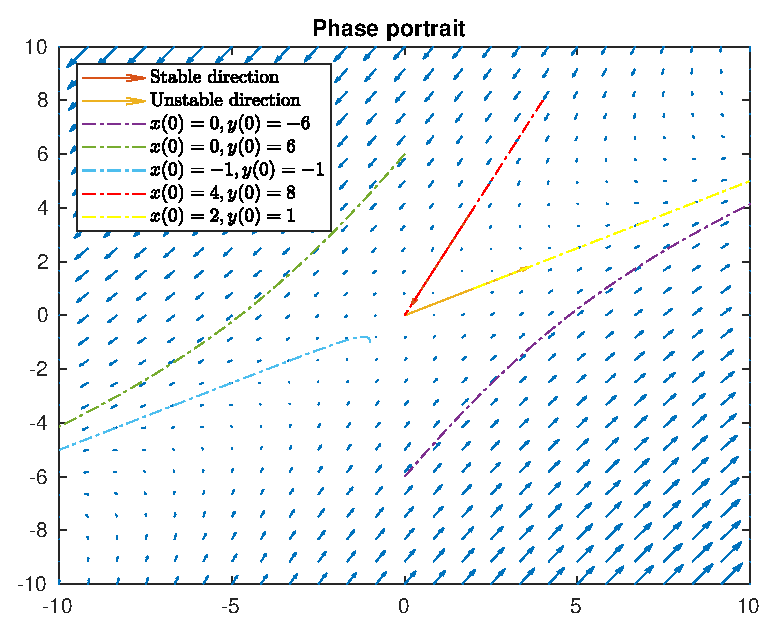
\includegraphics[width=\linewidth]{ODEsA3Q1f}
			\caption{Phase Portrait for the 2D system}
		\end{figure}

	\end{enumerate}
	\item The 2 population interaction model
	\[\dd{}t \begin{pmatrix}x\\y\end{pmatrix} = \begin{pmatrix}\alpha x + \beta xy\\ \gamma y + \delta xy\end{pmatrix}\]
	With
	\[\begin{cases}
		\alpha,\gamma > 0\\\beta,\delta < 0
	\end{cases}\]
	\begin{enumerate}
		\item %Write down the steady states (don't need to calculate) and for each of the steady states, determine the nature of the associated linearised problems 
				%We can just straight up use notes from lectures for this question
				From lectures the nullclines to this problem are
				\[\eta_x = \begin{cases}
					x=0,\\ y=-\alpha/\beta
				\end{cases} \]
				and
				\[\eta_y = \begin{cases}x = -\gamma/\delta,\\  y=0\end{cases}\]
				Hence the steady states are
				\[x=y=0, \quad \text{and}, \quad x=-\gamma/\delta,\, y=-\alpha/\beta\]
		\item %For each of the steady states for the non-linear system, state whether the behavious is equivalent to the linearised problem
		The steady states will behave like the linearised problem if they are \textit{hyperbolic equilibria}, i.e. if all the eigenvalues of the jacobian have non-zero real part. 
		Jacobian:
		\[J(x) = \begin{pmatrix}
			\alpha + \beta y&\beta x\\ \delta y& \gamma + \delta x
		\end{pmatrix}\]
		\[J(0,0) = \begin{pmatrix}
			\alpha&0\\ 0&\gamma
		\end{pmatrix}\]
		With eigenvalues $\lambda = \alpha,\gamma$ And we have assumed $\alpha,\gamma > 0$ so this will be equivalent to the linearised problem, and it will be unsteady. 

		\[J(-\gamma/\delta,-\alpha/\beta) = \begin{pmatrix}
			\alpha -\alpha & -\gamma\beta/\delta\\-\alpha \delta/\beta & \gamma - \gamma 
		\end{pmatrix} = \begin{pmatrix}
			0&-\gamma \beta/\delta\\ -\alpha \delta/\beta & 0
		\end{pmatrix}\]
		For the real part of both $\lambda's \neq 0$, i.e. neither of
		\begin{itemize}
		\item $tr\, J(x^*,y^*)=0 $ with $\det J(x^*,y^*) >0$, or
		\item $\det J(x^*,y^*) =0$
		\end{itemize}
		Since $tr\, J(x^*,y^*) =0$ require $\det J(x^*,y^*) < 0$ for nonzero real parts
		\begin{align*}
			\det J(x^*,y^*) &= -(-\gamma \beta/\delta)(-\alpha \delta/\beta)\\
			&= -\gamma \alpha
		\end{align*}
		Since $\gamma, \alpha > 1$ this means $\det J(x^*,y^*) <0$ and hence the linearised model will work, and the steady state will be a saddle.
		
		\item %State, with reason, if each of the states is biologically relevant
		The biologically relevant region is $x,y \geq 0$. $x=y=0$ is clearly in this region.
		$(-\gamma/\delta,-\alpha/\beta)$ is also in the region since $\alpha,\gamma>0, \beta,\delta <0$, and hence the state is for positive $x$ and $y$.
		\item %Produce a phase portrait, in the biologically relevant region of the phase plane, for the non-linear system with $\alpha = \gamma = 1$ and $\beta = \delta = -1$
		Figure~\ref{fig:phaseportrait2} shows the phase portrait for this non-linear system in the biologically relevant region. This region being $(x,y) > \mathbf{0}$.
		\begin{figure}[h]
			\centering
			\label{fig:phaseportrait2}
			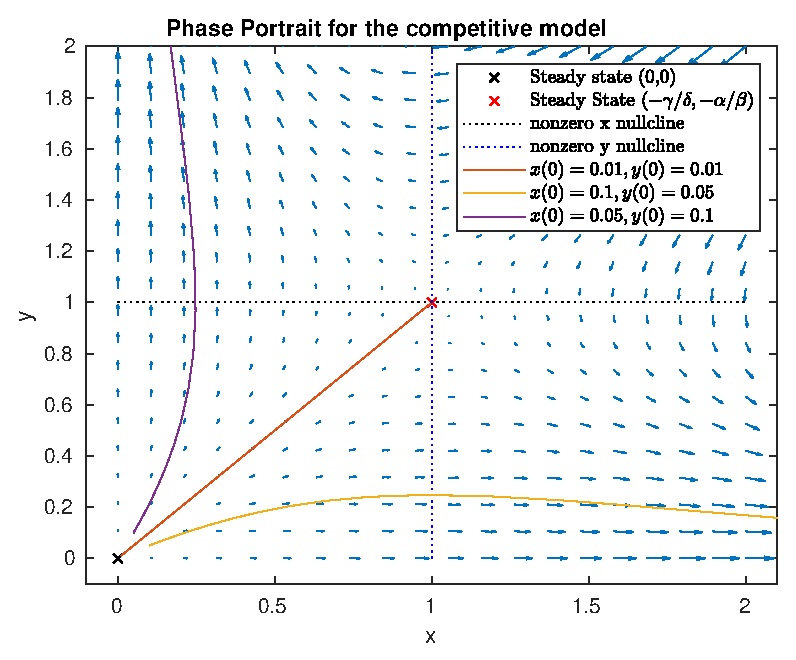
\includegraphics[width=\linewidth]{ODEsA3Q2d}
			\caption{Phase Portrait for the Competitive model}
		\end{figure}
		\item %Give a biological interpretation of the phase portrait
		This particular competitive model with $\alpha = \gamma = -\beta = -\delta$ is an even competition. When either population exceeds the other, they will continue to increase in number, and the other population will stagnate in number. If the populations remain equal (and non-zero, without perturbation), they will both increase up to the steady state $(-\gamma/\delta,-\alpha/\beta)$, which in this case is $(1,1)$. The phase portrait indicates that none of the steady states are stable.
	\end{enumerate}
\end{enumerate}
\clearpage
Matlab code:

\lstinputlisting{ODEsA3.m}


\clearpage
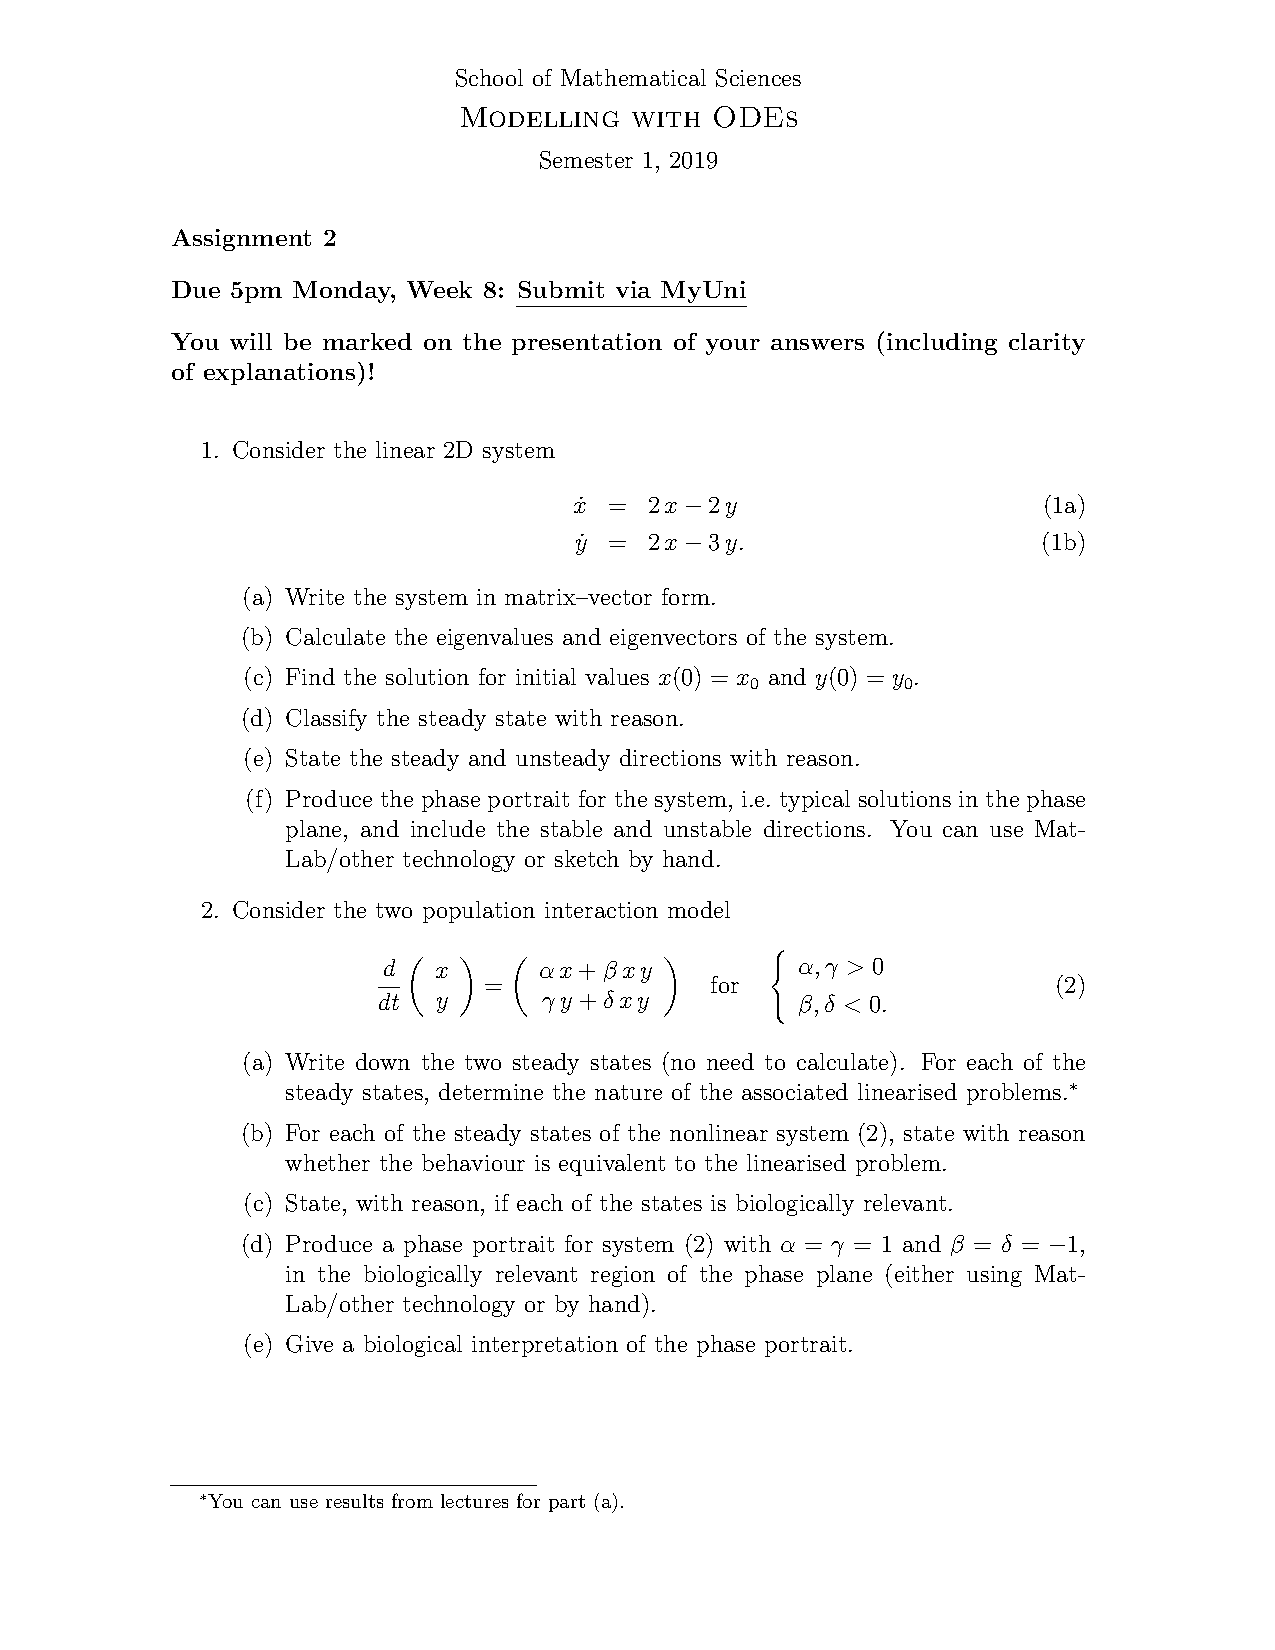
\includepdf{A3_2019.pdf}
\end{document}